\begin{figure}[h] % picture
	\centering
	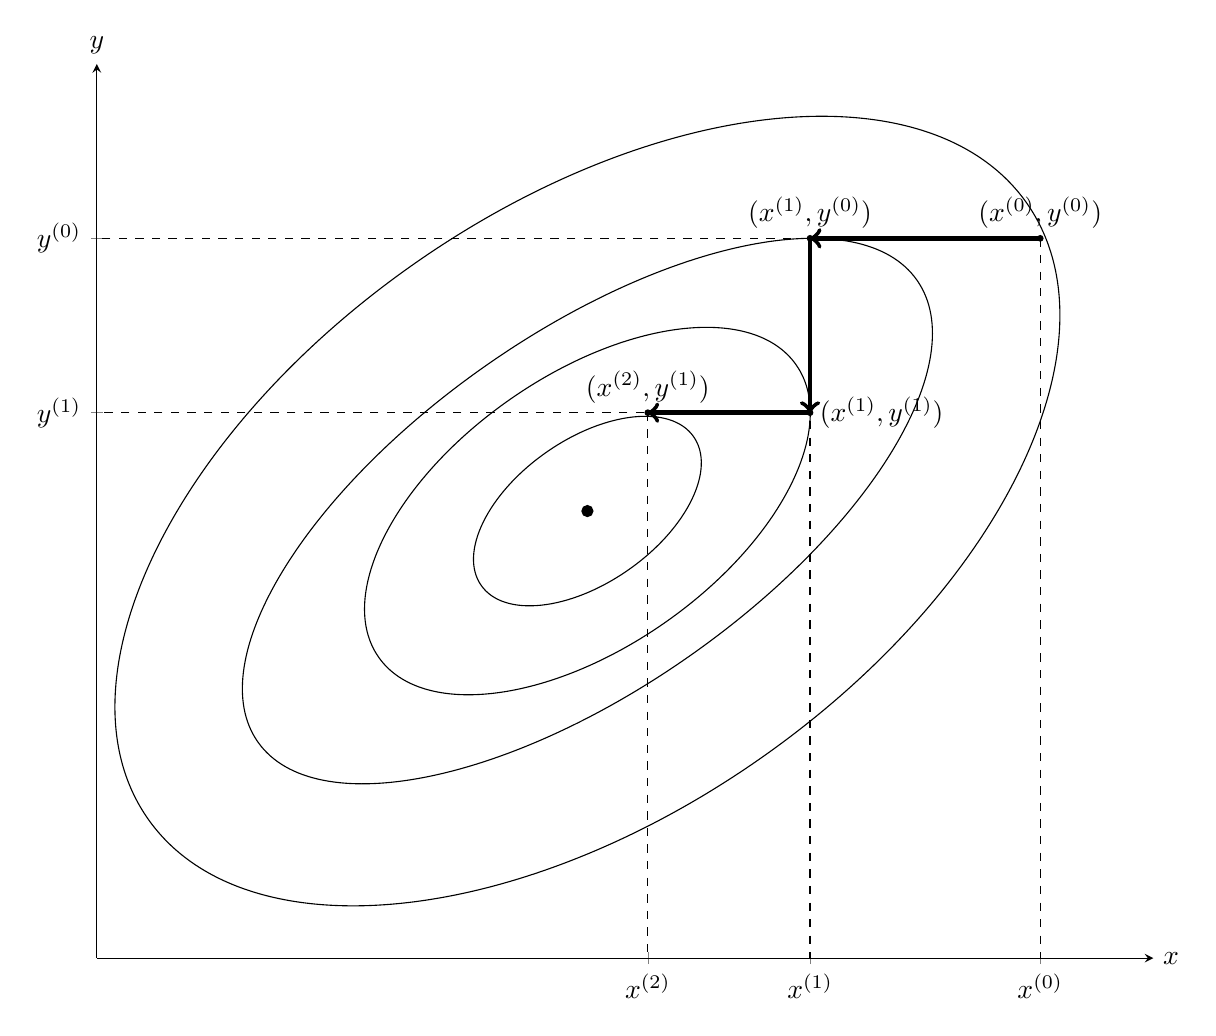
\begin{tikzpicture}
\begin{axis}[
	width = 15cm,
	xmin=-13,   xmax=15,
	ymin=-10,   ymax=10,
	axis y line*=left,
    axis x line*=bottom,
    axis lines = left,
	xtick={12, 5.9, 1.6},
	xticklabels = {$x^{(0)}$, $x^{(1)}$,$x^{(2)}$},
	ytick={6.1, 2.2},
	yticklabels = {$y^{(0)}$, $y^{(1)}$},
	        ylabel = {$y$}, ylabel style={rotate=-90},
        xlabel = {$x$},
        every axis x label/.style={
    		at={(ticklabel* cs:1.0)},
   			anchor=west,
			},
		every axis y label/.style={
    		at={(ticklabel* cs:1.0)},
    		anchor=south,
			}
]


	\draw[rotate around={-55:(0,0)},black] (0,0) ellipse (8 and 12);
	\draw[rotate around={-55:(0,0)},black] (0,0) ellipse (4.7 and 9);
	\draw[rotate around={-55:(0,0)},black] (0,0) ellipse (3.6 and 5.7);
	\draw[rotate around={-55:(0,0)},black] (0,0) ellipse (1.9 and 2.9);
	
	\addplot [only marks,mark=*] coordinates { (0,0) };

    
	\coordinate[label=above:{$(x^{(0)}, y^{(0)})$}] (A) at (12, 6.1);
	
	\draw[fill] (A) circle (1pt);
	\draw [dashed] (A) -- (A |- 0,-10);
	\draw [dashed] (A) -- (A -| -13,0);
	
	\coordinate[label=above:{$(x^{(1)}, y^{(0)})$}] (B) at (5.9, 6.1);
	
	\draw[fill] (B) circle (1pt);
	\draw [dashed] (B) -- (B |- 0,-10);
%	\draw [dashed] (B) -- (B -| -13,0);
	
	\coordinate[label=right:{$(x^{(1)}, y^{(1)})$}] (C) at (5.9, 2.2);
	
	\draw[fill] (C) circle (1pt);
%	\draw [dashed] (C) -- (C |- 0,-10);
	\draw [dashed] (C) -- (C -| -13,0);
	
	\coordinate[label=above:{$(x^{(2)}, y^{(1)})$}] (D) at (1.6, 2.2);
	
	\draw[fill] (D) circle (1pt);
	\draw [dashed] (D) -- (D |- 0,-10);
	
	\draw [->, ultra thick] (A) -- (B);
	\draw [->, ultra thick] (B) -- (C);
	\draw [->, ultra thick] (C) -- (D);
	
\end{axis}
\end{tikzpicture}
	\caption{Координатный спуск.}
	\label{fig:coordinate}
\end{figure}



\begin{figure}[h] % picture
	\centering
	\begin{tikzpicture}
\begin{axis}[
	width = 15cm,
	xmin=-13,   xmax=13,
	ymin=-10,   ymax=10,
	axis y line*=left,
    axis x line*=bottom,
    axis lines = left,
    domain=0:30,
    xtick={7.9, 1.9, -1.1},
	xticklabels = {$x^{(0)}$, $x^{(1)}$,$x^{(2)}$},
	ytick={7, 1, 4},
	yticklabels = {$y^{(0)}$, $y^{(1)}$, $y^{(2)}$},
	        ylabel = {$y$}, ylabel style={rotate=-90},
        xlabel = {$x$},
        every axis x label/.style={
    		at={(ticklabel* cs:1.0)},
   			anchor=west,
			},
		every axis y label/.style={
    		at={(ticklabel* cs:1.0)},
    		anchor=south,
			}
]

	\coordinate (O) at (-0.7, 2.8);
	\coordinate (O1) at (-2.1, 3.1);

	\draw[rotate around={-45:(0,0)},black] (0,0) ellipse (8 and 10);
	\draw[rotate around={-45:(O)},black] (O) ellipse (3.2 and 4);
	\draw[rotate around={-45:(O1)},black] (O1) ellipse (1 and 1.25);
%	
%	\draw[fill] (0, 0) circle (1pt);
%
    
	\coordinate[label=right:{$(x^{(0)}, y^{(0)})$}] (A) at (7.9, 7);
		\draw[fill] (A) circle (1pt);
		
	\addplot[dashed] {-x + 14.9}; % perpendicular is x
	
	\coordinate[label=right:{$(x^{(1)}, y^{(1)})$}] (B) at (1.9, 1);
		\draw[fill] (B) circle (1pt);
		
  	\draw[dashed] (A) -- (-0.1, -1); 
  	
  	\coordinate[label=right:{$(x^{(2)}, y^{(2)})$}] (C) at (-1.1, 4);
		\draw[fill] (C) circle (1pt);
		
	\draw[dashed] (B) -- (-3.1, 6); 
		
  	\draw[->, ultra thick] (A) -- (B);
  	\draw[->, ultra thick] (B) -- (C);
  	
  	
  	\draw [dashed] (A) -- (A |- 0,-10);
	\draw [dashed] (A) -- (A -| -13,0);
	
	\draw [dashed] (B) -- (B |- 0,-10);
	\draw [dashed] (B) -- (B -| -13,0);
	
	\draw [dashed] (C) -- (C |- 0,-10);
	\draw [dashed] (C) -- (C -| -13,0);
  	

	
\end{axis}
\end{tikzpicture}
	\caption{Градиентный спуск.}
	\label{fig:gradient}
\end{figure}


\begin{figure}[h] % picture
	\centering
	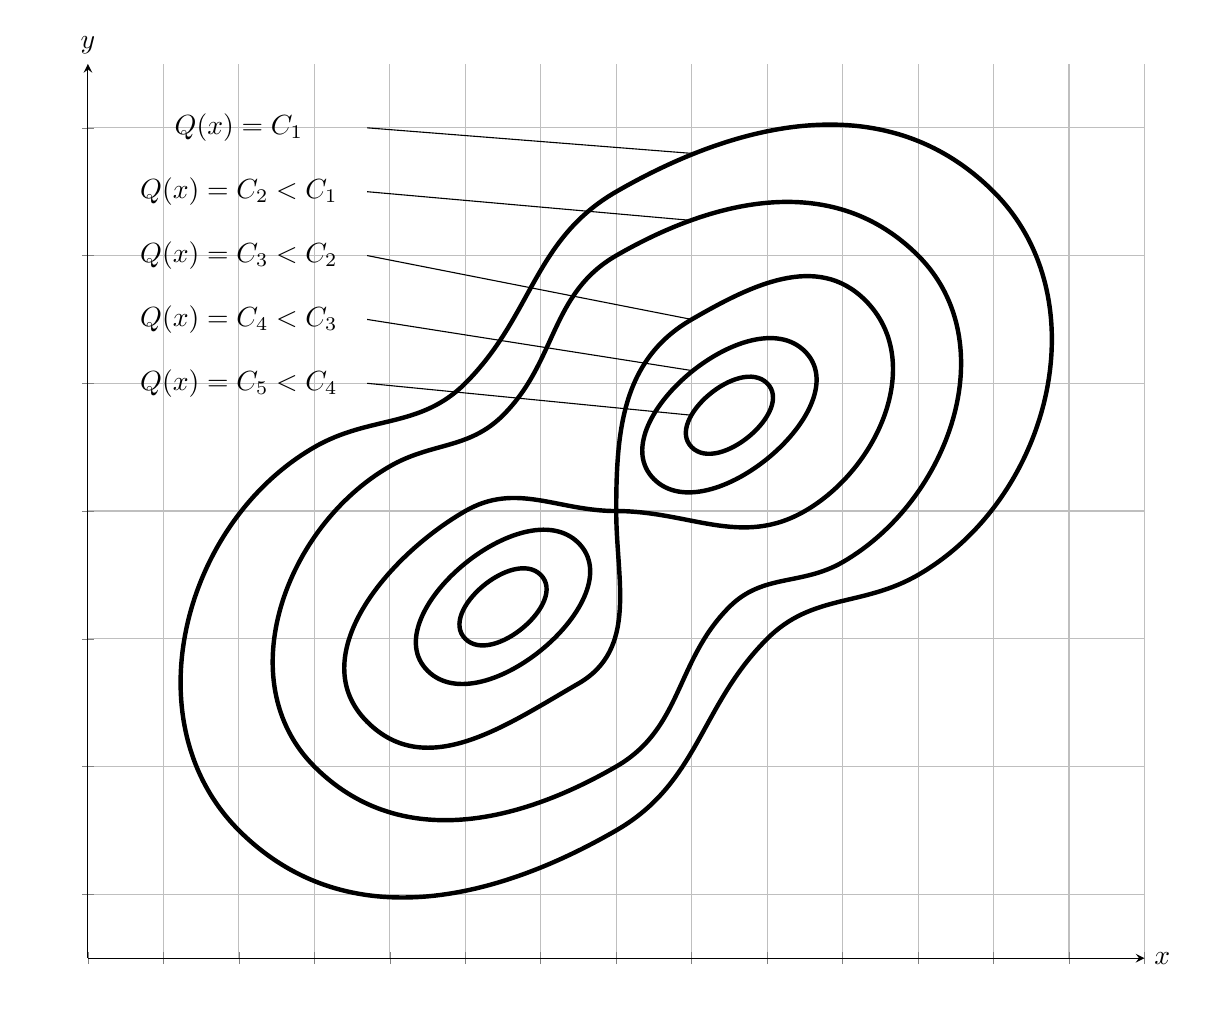
\begin{tikzpicture}
	
	\begin{axis}[
	width = 15cm,
	xmin=-7,   xmax=7,
	ymin=-7,   ymax=7,
	axis y line*=left,
    axis x line*=bottom,
    axis lines = left,
    domain=0:30,
    grid = major,
    tick label style = {white},
		    ylabel = {$y$}, ylabel style={rotate=-90},
        xlabel = {$x$},
        every axis x label/.style={
    		at={(ticklabel* cs:1.0)},
   			anchor=west,
			},
		every axis y label/.style={
    		at={(ticklabel* cs:1.0)},
    		anchor=south,
			}
]
 \draw [ultra thick,black] (5, 5 ) to[out=-45,in=30] (4, -1)
 		to[out=-150,in=45] (2,-2) to[out=-135,in=30] (0, -5)
 		to[out=-150,in=-45] (-5, -5)  to[out=135,in=-150] (-4, 1) 
 		to[out=30,in=-135] (-2, 2)  to[out=45,in=-150] (0, 5)
 		to[out=30,in=135] (5, 5) ;
 \draw [ultra thick,black] (4, 4 ) to[out=-45,in=30] (3, -0.8)
 		to[out=-150,in=45] (1.5,-1.5) to[out=-135,in=30] (0, -4)
 		to[out=-150,in=-45] (-4, -4)  to[out=135,in=-150] (-3, 0.7) 
 		to[out=30,in=-135] (-1.5, 1.5)  to[out=45,in=-150] (0, 4)
 		to[out=30,in=135] (4, 4)  ;
 \draw [ultra thick,black] (3.3, 3.3 ) to[out=-45,in=30] (2.5, 0)
 		to[out=-150,in=0] (0, 0)  to[out=90,in=-150] (1, 3)
 		to[out=30,in=135] (3.3,3.3)  ;
  \draw [ultra thick,black] (-3.3, -3.3 ) to[out=135,in=-150] (-2, 0)
 		to[out=30,in=180] (0, 0)  to[out=-90,in=30] (-0.5, -2.7)
 		to[out=-150,in=-45] (-3.3, -3.3) ;
 \draw [ultra thick,black] (2.5, 2.5) to[out=-45,in=-45] (0.5, 0.5) to[out=135,in=135] (2.5,2.5 );
  \draw [ultra thick,black] (2, 2) to[out=-45,in=-45] (1, 1) to[out=135,in=135] (2,2 );
  \draw [ultra thick,black] (-2.5, -2.5) to[out=-45,in=-45] (-0.5, -0.5) to[out=135,in=135] (-2.5,-2.5 );
  \draw [ultra thick,black] (-2, -2) to[out=-45,in=-45] (-1, -1) to[out=135,in=135] (-2,-2 );
  
  \node (A) at (-5, 6) {$Q(x) = C_1$};
  \draw (-3.3, 6) -- (1, 5.6);
  \node (B) at (-5, 5) {$Q(x) = C_2 < C_1$};
  \draw (-3.3, 5) -- (1, 4.55);
  \node (C) at (-5, 4) {$Q(x) = C_3 < C_2$};
  \draw (-3.3, 4) -- (1, 3.0);
  \node (D) at (-5, 3) {$Q(x) = C_4 < C_3$};
  \draw (-3.3, 3) -- (1, 2.2);
  \node (E) at (-5, 2) {$Q(x) = C_5 < C_4$};
  \draw (-3.3, 2) -- (1, 1.5);
\end{axis}
		
	\end{tikzpicture}
	\caption{Сложный ландшафт.}
	\label{fig:complex_landscape}
\end{figure}





\begin{figure}[h] % picture
	\centering
	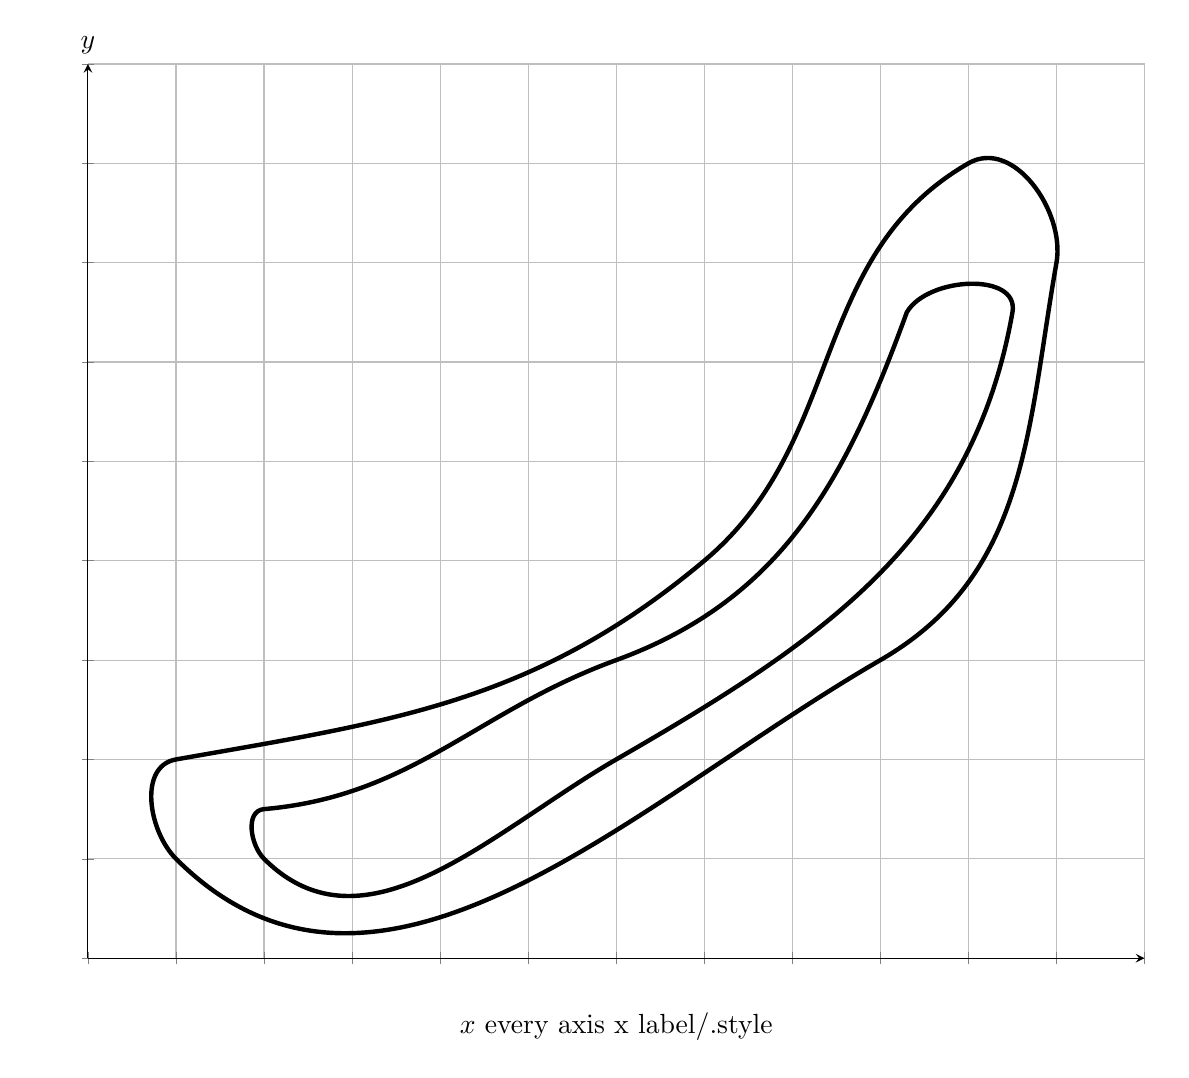
\begin{tikzpicture}
	
	\begin{axis}[
	width = 15cm,
	xmin=-5,   xmax=7,
	ymin=-2,   ymax=7,
	axis y line*=left,
    axis x line*=bottom,
    axis lines = left,
    domain=0:30,
    tick label style = {white},
    grid = major,
	    ylabel = {$y$}, ylabel style={rotate=-90},
        xlabel = {$x$}
        every axis x label/.style={
    		at={(ticklabel* cs:1.0)},
   			anchor=west,
			},
		every axis y label/.style={
    		at={(ticklabel* cs:1.0)},
    		anchor=south,
			}
]
 
 \draw [ultra thick,black] (-4, -1 ) to[out=-45,in=-150] (4, 1) to[out=30,in=-100] (6, 5)  to[out=80,in=30] (5, 6) to[out=-150,in=40] (2, 2) to[out=-140,in=10] (-4, 0) to[out=-170,in=135] (-4, -1)	 
 ;
 
 \draw [ultra thick,black] (-3, -1 ) to[out=-45,in=-150] (1, 0) to[out=30,in=-100] (5.5, 4.5)  to[out=80,in=60] (4.3, 4.5) to[out=-110,in=20] (1, 1) to[out=-160,in=5] (-3, -0.5) to[out=-175,in=135] (-3, -1)	 
 ;
		
\end{axis}
	\end{tikzpicture}
	\caption{Овраг}
	\label{fig:ovrag}
\end{figure}






